\documentclass{beamer}

\def\Tiny{\fontsize{6pt}{6pt}\selectfont}
\def\supertiny{\fontsize{4pt}{4pt}\selectfont}

\mode<presentation>
{
  \usetheme{Warsaw}
  % \setbeamercovered{transparent}
  \usecolortheme{crane}
}

\usepackage{graphicx, ifthen, listings, fancyvrb}

\usepackage[czech]{babel}
% \usefonttheme{professionalfonts}
\usepackage{times}
\usepackage{amsmath}
\usepackage[utf8]{inputenc}
\usepackage{wrapfig}

\usepackage[T1]{fontenc}

\lstset{ basicstyle=\tiny, stringstyle=\ttfamily, showstringspaces=false }

\everymath{\displaystyle}

\setbeamerfont{frametitle}{size=\large}
\setbeamerfont{subsection in toc}{size=\scriptsize}

\makeatletter\newenvironment{blackbox}{%
   \begin{lrbox}{\@tempboxa}\begin{minipage}{0.95\columnwidth}}{\end{minipage}\end{lrbox}%
   \colorbox{black}{\usebox{\@tempboxa}}
}\makeatother

\title[IMF (9)]{Informatika pro moderní fyziky (9)\\Tvorba textových dokumentů a vektorových obrázků}

\author[Franti\v{s}ek HAVL\r{U}J, ORF ÚJV Řež]{Franti\v{s}ek HAVL\r{U}J\\{\scriptsize \emph{e-mail: haf@ujv.cz}}}

\date{akademický rok 2019/2020\\20. listopadu 2019}

\institute[ORF ÚJV Řež]
{ÚJV Řež\\oddělení Reaktorové fyziky a podpory palivového cyklu}

\AtBeginSection[]
{
\begin{frame}<beamer>
\frametitle{Obsah}
\tableofcontents[currentsection,hideothersubsections]
\end{frame}
}

\begin{document}

\begin{frame}
  \titlepage
\end{frame}

\begin{frame}
  \tableofcontents
\end{frame}

\section{Co jsme se naučili minule}

\begin{frame}{}
  \begin{itemize}
    \item regulární výrazy
  \end{itemize}
\end{frame}

\section{Výroba dokumentu v~praxi - ERb}

\begin{frame}{Úkoly na dnešek}
  \begin{itemize}
    \item násobilku 10x10 z minula přepracovat tak, aby se vygenerovala 7x7, 9x9, 11x11 - použití parametrů v ERb
    \item přepracovat náš krásný report z JE Třeskoprsky s použitím ERb
    \item tabulky nicméně zajisté předělávat nebudeme
  \end{itemize}
\end{frame}

\begin{frame}[fragile]{Základní syntaxe ERb (1)}
  \begin{block}{ }
    Jakýkoli Ruby příkaz, přiřazení, výpočet ...
    \scriptsize
    \begin{verbatim}
      <% a = b + 5 %>
      <% list = ary * ", " %>
    \end{verbatim}
  \end{block}
\end{frame}

\begin{frame}[fragile]{Základní syntaxe ERb (2)}
  \begin{block}{ }
    Pokud chci něco vložit, stačí přidat rovnítko
    \scriptsize
    \begin{verbatim}
      <%= a %>
      <%= ary[1] %>
      <%= b + 5 %>
    \end{verbatim}
  \end{block}
\end{frame}

\begin{frame}[fragile]{Základní syntaxe ERb (3)}
  \begin{block}{ }
    Radost je možnost použít bloky a tedy i iterátory apod. v~propojení s~vkládaným textem:
    \scriptsize
    \begin{verbatim}
      <% (1..5).each do |i| %>
      Number <%= i %>
      <% end %>
      <% ary.each do |x| %>
      Array contains <%= x %>
      <% end %>
    \end{verbatim}
  \end{block}
\end{frame}

\begin{frame}{Co je podstatné}
  \begin{itemize}
    \item nezapomenout, kdy jsem v Ruby, kdy v ERb, kdy v latexu a vždy dodržet zadanou syntaxi
    \item mít na paměti, jak dostat data ze skriptu do šablony
    \item potřebuju mít načtený seznam všech kampaní do nějakého pole a to poslat do šablony
  \end{itemize}
\end{frame}


\section{Tvorba obrázků}

\begin{frame}{Zadání dnešní úlohy}
  \begin{itemize}
    \item pro zadanou textovou mapu AZ VR1 potřebuju udělat hezký obrázek
    \item co druh, to barvička, rozumně zacházet s odstíny (palivo různě modré, R/B/E tyče různě červené, zelené, fialové)
  \end{itemize}
\end{frame}

\begin{frame}{Jak na obrázky}
  \begin{itemize}
    \item pěkný formát na tvorbu vektorových obrázku je SVG (Scalable Vector Graphics)
    \item je to dobrá věc především na internet -- všechny prohlížeče ho umí
    \item stejně jako HTML je postaven na XML
  \end{itemize}
\end{frame}

\begin{frame}[fragile]{Jednoduchý příklad}
  \tiny
  \begin{verbatim}
    <svg width="320" height="320" xmlns="http://www.w3.org/2000/svg" version="1.1">
      <rect x="0.0" y="0.0" width="40.0" height="40.0" fill="blue" />
      <rect x="40.0" y="0.0" width="40.0" height="40.0" fill="red" />
      <rect x="0.0" y="40.0" width="40.0" height="40.0" fill="green" />
      <rect x="40.0" y="40.0" width="40.0" height="40.0" fill="yellow" />
    </svg>
  \end{verbatim}
  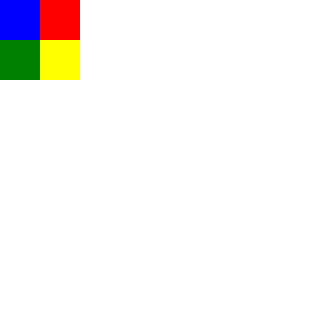
\includegraphics[width=0.15\textwidth]{example}
\end{frame}

\begin{frame}{SVG -- co a jak}
  \begin{itemize}
    \item souřadný systém z levého horního rohu
    \item je potřeba udat celkovou šířku a výšku
    \item zatím nám stačí obdélník -- tag \texttt{rect}
    \item pozor, je to striktní XML, tedy je nutné \texttt{rect} tag uzavřít (!)
    \item vyzkoušejte -- nejdřív jen tak, potom vygenerovat 8x8 mapu (zatím klidně prázdnou)
  \end{itemize}
\end{frame}

\begin{frame}{Další SVG chytrosti}
  \begin{itemize}
    \item kromě \texttt{rect} se bude hodit také \texttt{text}
    \item jako text se zobrazí obsah příslušného elementu
    \item opět použiju atributy \texttt{x}, \texttt{y} (levý dolní roh) a můžu přihodit \texttt{text-anchor=``middle''}, aby to byl dolní prostředek
  \end{itemize}
\end{frame}

\begin{frame}{Postup}
  \begin{itemize}
    \item načtu ze souboru třeba do 2D pole
    \item budu mít hash s barvičkama
    \item vykreslím do SVG
  \end{itemize}
\end{frame}

\begin{frame}{A to je vše, přátelé!}
  \begin{center}
    \includegraphics[width=0.8\textwidth]{looney_tunes}
  \end{center}
\end{frame}

\end{document}
